\documentclass[twocolumn,nofootinbib,showkeys,twoside,floatfix,unsortedaddress,flushbottom,12pt,aps,pra]{report}

%Some of this is probably not needed
\usepackage{amssymb,latexsym,amsmath,setspace}
%%\usepackage[colorlinks,linkcolor=blue]{hyperref}
\usepackage[colorlinks=true,allcolors=blue]{hyperref}
%%\usepackage[colorlinks]{hyperref}
%\usepackage{xspace}
%\usepackage{graphics,graphicx}
\usepackage{subfigure}
\usepackage{lineno}
\usepackage{fancyhdr}
\usepackage[english]{babel}  %% for texi2dvi ~ bug
%\usepackage[normalem]{ulem}
\usepackage[footnotesize,bf]{caption}
%\usepackage{placeins} % \FloatBarrier

\usepackage{tikz}
\usepackage{latexsym}% 
\usepackage{graphics,graphicx}
\usepackage{amssymb}% 
\usepackage{amsmath}
\usepackage{amsfonts} % mathbb
\usepackage{natbib}% 
\usepackage{fancyhdr,lastpage}
\usepackage{titlesec}
\usepackage{bold-extra}
%\usepackage[margin=0.7in,headheight=60pt]{geometry}
\usepackage[width = 18cm, height = 22cm,headheight=70pt, columnsep = 1cm]{geometry}

\usepackage{float}
\usepackage{listings}
\usepackage{subfigure}
\usetikzlibrary{shapes.geometric, arrows}
\tikzset{
  int/.style={circle, draw=black, fill=green!20, minimum size=3em},
  int1/.style={circle, draw=black, fill=red!20, minimum size=3em},
  int2/.style={circle, draw=black, fill=blue!20, minimum size=3em},
  init/.style={pin distance=1.2cm,pin edge={loop,thin,black}}
}
\tikzstyle{arrow} = [thick,black,->,>=stealth]
\tikzstyle{pinstyleto} = [pin edge={<-,thick,black}]
\tikzstyle{pinstyleout} = [pin edge={->,thick,black}]


\newcommand\numberthis{\addtocounter{equation}{1}\tag{\theequation}}


\AtBeginDocument{%
\renewcommand{\thesection}{\arabic{section}}%
\renewcommand{\contentsname}{\sc{\bfseries Contents}}
\renewcommand{\bibname}{\sc{\bfseries Bibilography}}
}



\author{\sc{\bfseries Group 2:}\\
\small \emph{Nicole Sandra-Yaffa Dumont \footnote{ns2dumon@uwaterloo.ca}} \\
 \small \emph{Sakif Hossain Khan \footnote{sh9khan@uwaterloo.ca}} \\
 \small  \emph{Kira Aveline Selby \footnote{kaselby@uwaterloo.ca}} \\
 \small  \emph{Congcong Zhi \footnote{c3zhi@edu.uwaterloo.ca}} } 
 
 \title{ \small \emph{STAT 841/ CM 763: Statistical Learning - Classification }\\
  \Huge \sc{\bfseries Constructing Textual Artificial Conversational Entities using Deep Learning}}
  \date{\small \today }
  

%\renewcommand{\abstractname}{\Huge \sc{Executive Summary}}

  \titleformat{\section}
  {\centering \normalfont \bfseries \scshape }{\thesection}{1em}{}
  
  \titleformat{\subsection}
  {\centering \normalfont \itshape \bfseries}{\thesubsection}{1em}{}


%Optional headers
\lhead{\sc{}}
\rhead{\emph{}} 

\renewcommand\headrulewidth{0pt}% Removes funny header line
\begin{document}



\pagestyle{fancy}

\maketitle
\tableofcontents

\onecolumn
\section*{\Huge Executive Summary}
\addcontentsline{toc}{section}{\protect\numberline{}Executive Summary}% 

a summary



\twocolumn

\section{Abstract} 
an abstract
\par \smallskip \qquad

\section{Background}
some background \par
\smallskip

\section{Methods}
\subsection{Recurrent Neutral Networks (RNNs)} 
\indent
an example flow chart
\begin{center}
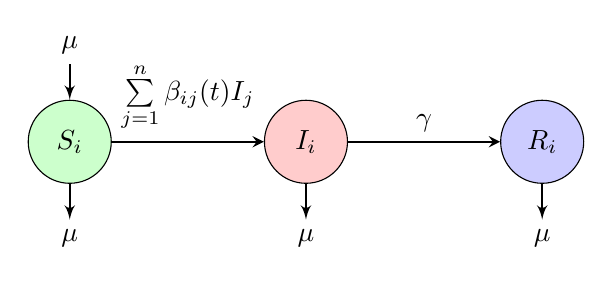
\begin{tikzpicture}[node distance=3cm,auto,>=latex',every node/.append style={align=center}]
    \node [int, pin={[pinstyleto]above:$\mu$}, pin={[pinstyleout]below:$\mu$}] (a)              {$S_i$};
    \node [int1, pin={[pinstyleout]below:$\mu$}] (b) [right of=a] {$I_i$};
    \node [int2, pin={[pinstyleout]below:$\mu$}] (c) [right of=b] {$R_i$};
    
    \draw [arrow] (a) -- node[anchor=south] {$ \sum\limits_{j=1}^{n}\beta_{ij}(t) I_j $} (b);
    \draw [arrow] (b) -- node[anchor=south] {$\gamma$} (c);
\end{tikzpicture}
\end{center}

\subsection{The seq2seq Model} 


\section{Results}
results go here

\section{Conclusion} 
a conclusion

\onecolumn
\addcontentsline{toc}{section}{\protect\numberline{}Bibilography}%
\bibliographystyle{unsrt}
%uncomment once we have a bib file
%\bibliography{bibfilename} 
\end{document}
